\chapter[Sweeper]{Sweeper: ejecución de flujos de trabajo en cómputo en la nube}
\label{chap:sweeper}

En este capítulo se describen los detalles del funcionamiento de Sweeper \cite{dominofire2015sweeper}, el sistema de administración de flujos de trabajo orientado a cómputo en la nube. Utilizando este paquete, se pueden ejecutar tareas expresadas como comandos de una terminal Linux, con dependencias de orden entre estas tareas, ejecutadas remotamente en m\'aquinas virtuales en la nube. Sweeper está desarrollado en el lenguaje de programación Python \cite{python3}.

Para ejecutar flujos de trabajo con Sweeper, se especifican las tareas del flujo de trabajo y sus dependencias. Sweeper lee este archivo de descripción y enseguida estima los tiempos de ejecución de las tareas y elige la mejor asignación de máquinas virtuales y tareas del flujo de trabajo que optimicen los criterios dados.

Para crear un flujo de trabajo, se crea un archivo que cumpla con el formato YAML \cite{dot2015yaml} llamado \texttt{workflow.yaml}. De esta forma, en la sección \texttt{workflow}, se definen, en forma de lista, las tareas que conforman el flujo de trabajo. En el código \ref{code:workflow_example} se puede apreciar la estructura del archivo del flujo de trabajo.  

\begin{lstlisting}[label={code:workflow_example},caption={Flujo de trabajo de ejemplo.},float]
workflow:
  - name: check_files
    command: ls -alp

  - name: create_filelist
    command: ls -alp > sal.txt
    depends: [check_files]
    download_files: [sal.txt]

  - name: create_sysinfo
    command: lsb_release -a > info.txt
    depends: [check_files]

  - name: final_results
    command: ls -alp
    depends: [create_filelist, create_sysinfo]
\end{lstlisting}

En el listado de código \ref{code:workflow_example} se muestra la descripcion de un flujo de trabajo que imprime los nombres de los archivos contenidos en las máquinas virtuales que ejecutan este flujo. También, este flujo trabajo contiene una tarea para recolectar la información de la versión del sistema operativo que ejecuta la máquina virtual. Por otro lado, en la figura \ref{fig:workflow_test} se encuentra la representación visual de este flujo de trabajo. 

\begin{figure}
\begin{center}
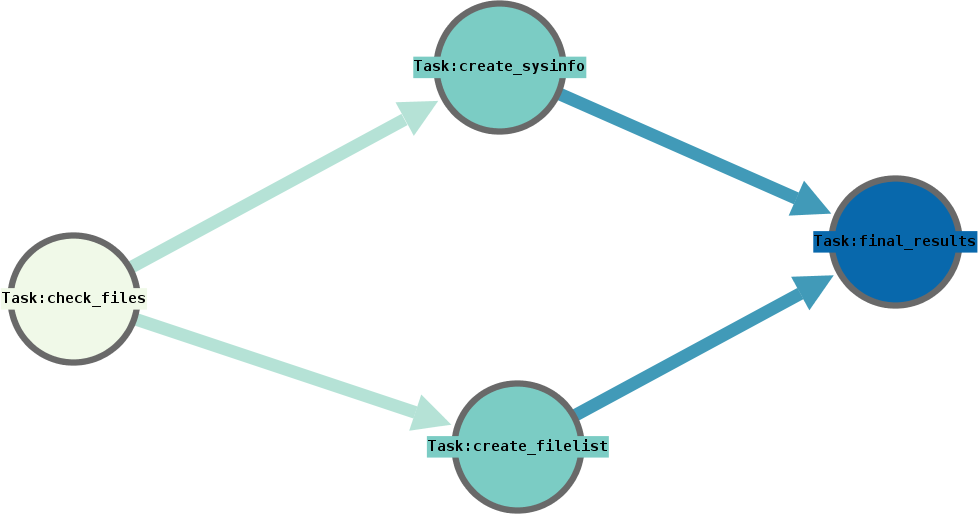
\includegraphics[width=0.8\textwidth]{imagenes/workflow_test.png}
\end{center}
\caption{Visualización del flujo de trabajo \emph{test} }
\label{fig:workflow_test}
\end{figure}


En el ejemplo anterior se pueden apreciar los elementos básicos que componen una tarea del flujo de trabajo, los cuales son explicados a continuación:


\begin{itemize}
\item{\texttt{name}: Nombre de la tarea, que es único entre los nombres de las demás tareas del flujo de trabajo.}
\item{\texttt{command}: Comando en sintaxis de Bash que será ejecutado en esta tarea.}
\item{\texttt{depends}: Lista de los nombres de las tareas que necesitan ser ejecutadas antes de que esta tarea pueda ejecutarse.}
\item{\texttt{download\_files}: Lista de los archivos que deben ser descargados después de terminar la ejecución de la tarea.}
\item{\texttt{include\_files}: Lista de los archivos que deben ser subidos al cluster antes de que la tarea sea ejecutada.}
\end{itemize}

Una característica importante de Sweeper que lo hace único a otros sistemas de administración de flujos de trabajo, es la expansión de parámetros. El usuario puede especificar una tarea que se requiera ejecutar con un conjunto predefinido de argumentos. Sweeper calcula todas las combinaciones posibles de parámetros y automáticamente crea una tarea a ejecutarse por cada posible combinaci\'on de parámetros. Esto es de gran utilidad para la ejecución de experimentos y para la ejecución de aplicaciones de barrido de parámetros. Así, en el listado del código \ref{code:forests_2} se muestra un flujo de trabajo que utliza listas de parámetros de donde se generan las combinaciones de argumentos. En la figura \ref{fig:workflow_forests} se encuentra la representación gr\'afica de este flujo de trabajo.

\begin{figure}
\begin{center}
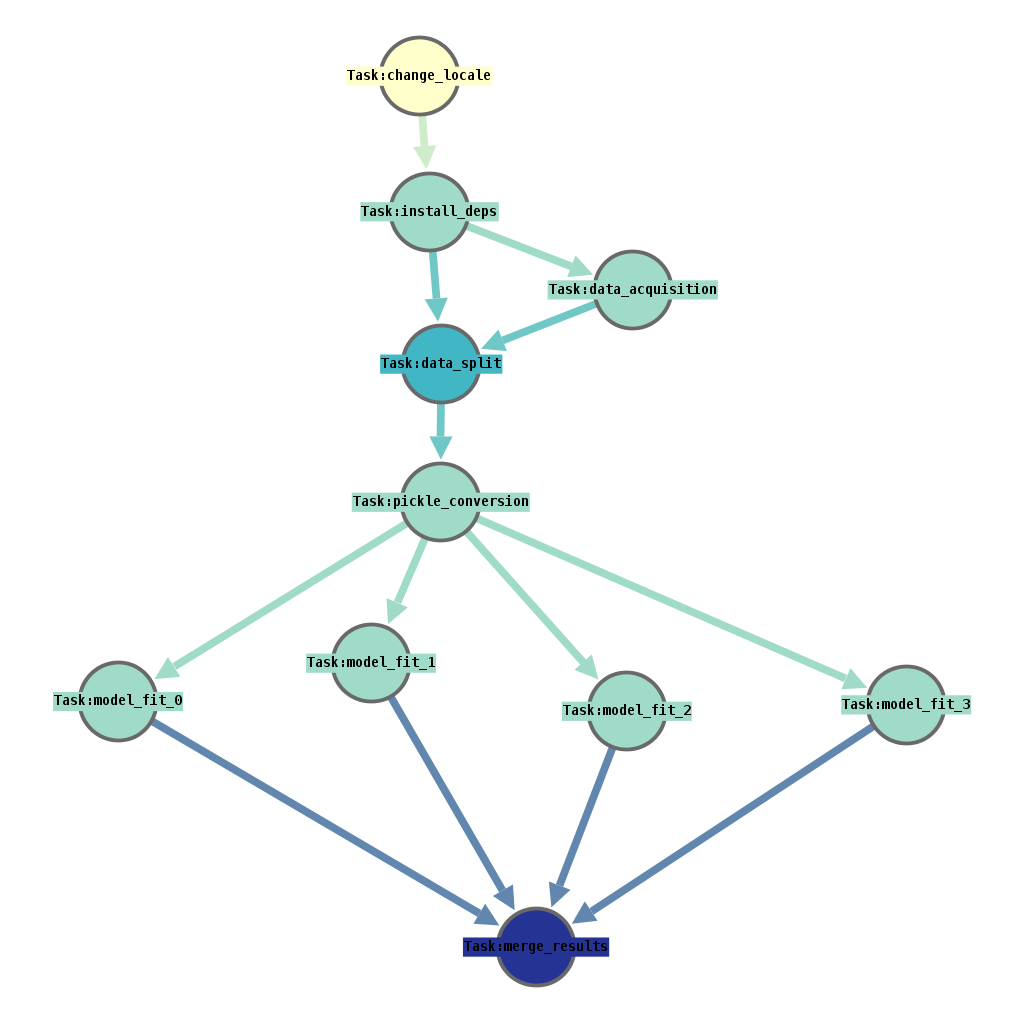
\includegraphics[width=0.8\textwidth]{imagenes/workflow_forests.png}
\end{center}
\caption{Visualización del flujo de trabajo \emph{forests} }
\label{fig:workflow_forests}
\end{figure}

\begin{lstlisting}[label={code:forests_1},caption={Flujo de trabajo para búsqueda de parámetros (parte 1).},float]
workflow:
  - name: change_locale
    command: |
        echo "LC_ALL=en_US.UTF-8" | sudo tee -a /etc/environment;
        echo "LANG=en_US.UTF-8" | sudo tee -a /etc/environment;
        sudo update-locale LANG=en_US.UTF-8 LC_ALL=en_US.UTF-8;

  - name: install_deps
    command: |
        set -o xtrace;
        # scikit-learn
        export DEBIAN_FRONTEND=noninteractive;
        sudo apt-get update;
        sudo apt-get install unzip -y;
        sudo apt-get install build-essential gfortran gcc g++ \
                        python3-dev python3-pip python3-setuptools \
                        python3-numpy python3-scipy python3-matplotlib \
                        libatlas-dev libatlas-base-dev libatlas3gf-base -y;
        sudo update-alternatives --set libblas.so.3 /usr/lib/atlas-base/atlas/libblas.so.3;
        sudo update-alternatives --set liblapack.so.3 /usr/lib/atlas-base/atlas/liblapack.so.3;
        sudo pip3 install -U scikit-learn;
        # doge package
        sudo apt-get install git -y;
        git clone https://github.com/dominoFire/doger.git;
        cd doger;
        sudo pip3 install .;
        cd ..;
    depends: [change_locale]

  - name: data_acquisition
    command: |
        unzip train.csv.zip;
        mv train.csv labeled.csv;
    include_files: [train.csv.zip]
    depends: [install_deps]

  - name: data_split
    command: |
        doger split_traintest labeled.csv 0.70;
        doger split_xy labeled_train.csv Cover_Type;
        doger split_xy labeled_test.csv Cover_Type;
    depends: [data_acquisition, install_deps]

  - name: pickle_conversion
    command: |
        doger csv2pk labeled_train_predictors.csv labeled_train_response.csv;
        doger csv2pk labeled_test_predictors.csv labeled_test_response.csv;
    depends: [data_split]
\end{lstlisting}

\begin{lstlisting}[label={code:forests_2},caption={Flujo de trabajo para búsqueda de parámetros (parte 2).},float]
  - name: model_fit
    command: |
        doger gridsearch \
            labeled_train_predictors.pk labeled_train_response.pk \
            labeled_test_predictors.pk labeled_test_response.pk \
            @config_file \
            obj out;
    depends: [pickle_conversion]
    param_grid:
        config_file: [gridsearch_xt_config.py, gridsearch_rf_config.py, gridsearch_gnb_config.py, gridsearch_bnb_config.py]
    include_files: [gridsearch_xt_config.py, gridsearch_rf_config.py, gridsearch_gnb_config.py, gridsearch_bnb_config.py]

  - name: merge_results
    command: |
        doger merge out;
    depends: [model_fit]
    download_files: [out/AllResults.csv]
\end{lstlisting}


\section{Arquitectura}

En figura \ref{fig:sweeper-arch} se muestra la arquitectura de Sweeper, en donde se pueden los grandes componentes: la ejecución del flujo de trabajo y el planificador. Sweeper utiliza las interfaces de programación de aplicaciones de cada proveedor de servicios de cómputo en la nube para reservar, ejecutar y administrar los recursos utilizados en la nube de cada proveedor. Actualmente, Sweeper puede trabajar con los servicios de cómputo en la nube de Microsoft Azure \cite{microsoft2015azure}. En las siguientes subsecciones, describiremos a detalle cada uno de los componentes de Sweeper.

\begin{figure}
\begin{center}
%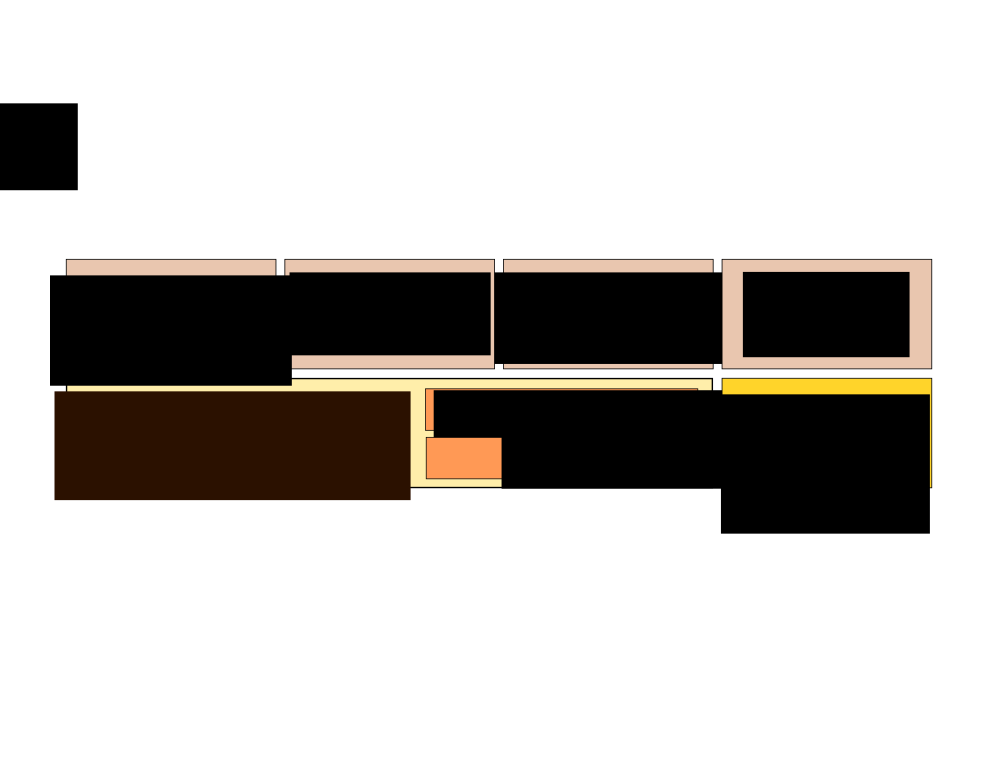
\includegraphics[width=0.8\textwidth]{imagenes/sweeper-architecture.pdf}
\end{center}
\caption{Arquitectura de Sweeper}
\label{fig:sweeper-arch}
\end{figure}


\subsection{Ejecución de flujos de trabajo}

Este componente se encarga de ejecutar el flujo de trabajo en los recursos en la nube de acuerdo a la planificación generada por el componente de planificación. Por el momento, este componente implementa un sistema de colas concurrente en las que las tareas son insertadas y despachadas de acuerdo al tiempo de ejecución estimado.



\subsection{Planifcador}

El planificador busca la asignación de recursos que optimice la calidad en el servicio en la ejecución del flujo de trabajo, interpretado como restricciones de presupuesto o restricciones de fechas límite. 



% \subsection{Perfilador de tareas}

% El perfilador de tareas se utiliza para obtener un modelo de la estimación de tiempos de ejecución independiente de la máquina, el cual es útil para generar planificaciones que optimicen el tiempo total de ejecución o el presupuesto utilizado para la ejecución del flujo de trabajo. A grandes rasgos, el Perfilador de tareas mide el tiempo de ejecución de cada tarea de un flujo de trabajo, guardando un registro de estos tiempos de ejecución junto con los parámetros que se utilizaron para invocar cada tarea.

% Para utilizar el perfilador, hay que invocar Sweeper con la opción \texttt{profile} en la carpeta en donde se encuentre el archivo de flujo de trabajo (\texttt{workflow.yaml}) que se quiera ejecutar, de la siguiente forma:

% \begin{lstlisting}[language=bash]
% $ sweeper profile
% \end{lstlisting}


% \subsection{Perfilador de recursos}

% También, para estimar la velocidad de las máquinas virtuales de un proveedor, sweeper se auxilia del PerfKitBenchmarker, un software diseñado para correr benchmarks, los cuales son pruebas de estrés que ejecutan las máquinas virtuales, cuyos resultados son analizados posteriormente. Para el caso de Sweeper, se utilzan las mediciones de FLOPS que provee el benchmark SPECfp.

